\documentclass[11pt]{article}
\usepackage[margin=1in]{geometry}
\usepackage{amsmath,amssymb,amsthm,mathtools}
\usepackage{booktabs,graphicx,array}
\usepackage{hyperref}
\usepackage[round]{natbib}
\hypersetup{colorlinks=true,linkcolor=blue,citecolor=blue,urlcolor=blue}
\newtheorem{proposition}{Proposition}
\newtheorem{remark}{Remark}
\newcommand{\one}{\mathbf{1}}
\newcommand{\EE}{\mathbb{E}}
\newcommand{\QQ}{\mathcal{Q}}
\title{Research Note: Transport Bounds for Conditional and Path-Dependent Event Contracts}
\author{Derivative Parity Research --- working manuscript}
\date{October 29, 2026 \quad (synthetic pilot; not a completed empirical paper)}
\begin{document}
\maketitle
\begin{abstract}
We formulate finite-state, model-robust bounds for binary, conditional, and
path-dependent event contracts using linear programming, multi-marginal optimal
transport, and (where the event depends on a dynamically traded asset)
martingale optimal transport. The distinction between static consistency and
dynamic self-financing hedging is central. Three reproducible \emph{synthetic}
examples yield: a three-event intersection price in $[0.15,0.22]$; a
rally-then-decline price in $[1/12,1/4]$ under martingale constraints, versus
$[0,1/2]$ under ordinary couplings; and a three-date
rally-decline-rebound price in $[0,1/16]$ versus $[0,1/4]$. Explicit rational
primal and pathwise dual certificates certify these finite examples.
They are demonstrations rather than claims of new theoretical results.
We state a falsifiable empirical research agenda for assessing interval
contraction and executable violations using settlement-aligned cross-market data.
\end{abstract}

\section{Economic interpretation and identification}
A unit-collateralized binary claim has payoff $H\colon\Omega\to\{0,1\}$,
where $\Omega$ is an explicit, common set of settlement states. If all
contracts share a numeraire, settlement time and consistent pricing measure
$Q$, their normalized present values are $\EE_Q[H]$. These are
\emph{pricing-measure} expectations, not automatically physical probabilities.
Differences in oracle criteria, observation windows, collateral, fees,
settlement delays and tradeability invalidate naive cross-market parity.
A static price interval is a \emph{consistency bound} under the hypotheses,
not automatically a directly executable arbitrage.
The admissible laws in this note may assign zero mass to settlement states.
They are not assumed equivalent to a specified physical reference measure.

Conditional-token positions can be intersections of distinct conditions, but
a position paying on $A\cap B$ is not itself a normalized conditional claim
paying $\one_B$ given $A$. Where $Q(A)>0$, $Q(B\mid A)=Q(A\cap B)/Q(A)$,
with careful treatment of the conditional settlement mechanism
\citep{gnosisconditional}. Prices $Q(B\mid A)$ and $Q(A\cap B)$ cannot be
interchanged.

\section{Finite-state transport and its dual}
Let $\Omega=\{\omega_1,\ldots,\omega_N\}$, $q_i=Q(\omega_i)$, and let
$h_j(\omega)$ be observed contract payoffs. With observed executable or
modeling quote intervals $[\ell_j,u_j]$, consider
\begin{align}
\QQ=\bigl\{q\in\mathbb R_+^N:\; &\one^\top q=1,\quad
\ell_j\le h_j^\top q\le u_j\ (j=1,\ldots,m),\\
& Dq=0\bigr\},
\end{align}
where $D$ optionally encodes structural restrictions. The sharp robust
interval for target payoff $H$, assuming $\QQ$ is nonempty, is
\begin{equation}
\underline\pi(H)=\min_{q\in\QQ}H^\top q,\qquad
\overline\pi(H)=\max_{q\in\QQ}H^\top q.
\label{eq:bounds}
\end{equation}
Here $\mathbb R_+^N$ means $q_i\ge0$, so the feasible set is closed and
the extrema are attained. Equivalence $Q\sim P$ to a full-support reference
law $P$ would require $q_i>0$ on every atom. The strictly positive class
need not attain its bounds: one must use infimum and supremum there.
If a feasible full-support law $q_*$ exists, mixing it with any feasible
boundary law preserves the linear constraints and approaches that boundary.
Only under this additional existence hypothesis do the two classes have
the same extremal values; endpoint attainment is a separate question.
For exact quotes $h_j^\top q=p_j$ and $D=0$, finite-dimensional LP duality
yields
\begin{align}
\overline\pi(H)=\min_{a_0,a}&\quad a_0+\sum_j a_jp_j
\quad\text{s.t.}\quad a_0+\sum_j a_jh_j(\omega)\ge H(\omega),\quad\forall\omega.
\end{align}
The lower dual replaces ``$\min$'' by ``$\max$'' and ``$\ge$'' by ``$\le$''.
A dual solution is a statewise sub/super-replicating portfolio. Inequality
quotes require the complete inequality dual; one cannot simply reuse the
exact-quote hedge coefficients. General theory is developed by
\citet{beiglbock2013model}.

\section{Example I: joint and conditional binary claims}
Let $A,B,C$ be binary outcomes observed at three monitoring dates and
assume the following \emph{hypothetical, normalized} price constraints:
\begin{equation}
(p_A,p_B,p_C,p_{AB},p_{BC},p_{AC})=(.60,.55,.45,.40,.30,.22).
\end{equation}
Let $q=Q(A\cap B\cap C)$. Inclusion-exclusion and monotonicity imply
\begin{equation}
0.15=p_{AB}+p_{BC}-p_B\le q\le p_{AC}=0.22.
\end{equation}
These bounds are sharp: explicit rational eight-state distributions attain
both endpoints, and exact arithmetic checks the dual inequalities
\begin{equation}
\one_{AB}+\one_{BC}-\one_B\le\one_{ABC}\le\one_{AC}.
\end{equation}
In lexicographic state order $000,001,010,011,100,101,110,111$, the endpoint
mass vectors are
\[
q^-=(17,8,0,15,13,7,25,15)/100,\qquad
q^+=(10,15,7,8,20,0,18,22)/100.
\]
Both are nonnegative, sum to one and satisfy all six quote equations.
For an explicit equivalence check, put $x=Q(ABC)$. All admissible masses are
\[
q(x)=(.32-x,\ x-.07,\ x-.15,\ .30-x,\ x-.02,\ .22-x,\ .40-x,\ x).
\]
Thus all eight masses are positive exactly when $.15<x<.22$.
The endpoint laws have respectively zero mass at 010 and 101, and are not
equivalent to full-support $P$. For $0<t<1$, $(1-t)q^-+tq^+$ is strictly
positive and has target value $.15+.07t$. Hence $.15$ and $.22$ remain
the infimum and supremum under equivalence, but neither is attained there.
This algebraic demonstration is separate from the compiled nonnegative-law
theorem; no Lean equivalence theorem is claimed.
No martingale assumption is made for these Boolean events, including
nontradable news, election or sports outcomes.
The synthetic input $p_{AB}=0.40$ fixes the conditioning denominator, hence
$Q(C\mid A\cap B)\in[0.375,0.55]$. With only the three marginals,
the interval for $Q(ABC)$ is $[0,0.45]$. With $AB$ and $BC$ added,
it shrinks to $[0.15,0.30]$.
In the full-support six-quote class the conditional range is instead
$(0.375,0.55)$, since the denominator remains $0.40$.

\section{Example II: a two-date price-path digital}
Here the state is a \emph{tradable}, appropriately discounted asset price,
with zero interest, payouts and funding adjustments in the synthetic model.
Prescribe
\begin{align}
S_1&\in\{90,110\}, &Q(S_1=90)=Q(S_1=110)&=\tfrac12,\\
S_2&\in\{70,90,110,130\}, &Q(S_2=s)&=\tfrac14\quad\text{for each }s.
\end{align}
The target is a monitored rally followed by a decline:
\begin{equation}
H=\one_{\{S_1=110\}}\one_{\{S_2\le90\}}.
\end{equation}
Ordinary OT over couplings of the two marginals yields $[0,1/2]$. The
martingale restriction $\EE_Q[S_2\mid S_1]=S_1$ leads to a smaller interval.
\begin{proposition}
For the two marginals above, among martingale couplings the sharp prices of
$H$ are $\underline\pi(H)=1/12$ and $\overline\pi(H)=1/4$.
\end{proposition}
\begin{proof}
Write $u=Q(110,70)$, $v=Q(110,90)$, $w=Q(110,110)$ and
$z=Q(110,130)$. The row sum and conditional martingale equation are
\begin{equation}
u+v+w+z=\tfrac12,\qquad -40u-20v+20z=0.
\end{equation}
Thus $z=2u+v$ and $w=\tfrac12-3u-2v$. Each column has mass $1/4$,
so $z\le1/4$ and $w\le1/4$. Consequently
$u+v\le z\le1/4$ and
$3(u+v)\ge3u+2v\ge1/4$, yielding
$1/12\le u+v\le1/4$.
For the lower endpoint, take the joint row masses (not conditional probabilities)
$(u,v,w,z)=(1/12,0,1/4,1/6)$; for the upper endpoint take
$(0,1/4,0,1/4)$. Subtracting these rows from the respective column
marginals yields nonnegative complementary rows. Since the unconditional
mean of $S_2$ equals that of $S_1$, the remaining row is a martingale too.
Both bounds are attained.
\end{proof}
Attainment here allows zero joint masses. The midpoint of the two endpoint
laws is the strictly positive feasible martingale law
\[
q_*=(5,3,3,1,1,3,3,5)/24.
\]
If full support is required, then $u,v>0$ and $w,z<1/4$, so
\[
u+v<z<1/4,\qquad 3(u+v)=1/2-w+v>1/4.
\]
The values $1/12$ and $1/4$
are then unattained infimum and supremum, approached by positive mixtures.
\begin{proposition}[Explicit sub- and superhedges]
Let $G=\one_{\{S_1=110\}}(S_2-S_1)$ be the gain on a predictable
self-financing position in the discounted underlying. Then for every
permitted pair $(S_1,S_2)$,
\begin{align}
\underbrace{\tfrac13\one_{\{S_1=110\}}-
\tfrac13\one_{\{S_2=110\}}-\tfrac1{60}G}_{L}
\le H\le
\underbrace{\one_{\{S_2=130\}}-\tfrac1{20}G}_{U}.
\end{align}
The costs of $L$ and $U$ are $1/12$ and $1/4$, respectively.
\end{proposition}
\begin{proof}
Check the eight possible $(S_1,S_2)$ states. The martingale
condition implies $\EE_Q[G]=0$, while the observed marginals price
the digital terms at $1/2$ and $1/4$. Equality of the optimal values
follows from the extremal couplings above. The test suite checks both
pointwise inequalities and all equality constraints.
\end{proof}
A further \emph{hypothetical} joint quote
$Q(S_1=110,S_2=130)=0.20$ shrinks the martingale interval to $[0.10,0.20]$.
This quote is a modeling input in the toy experiment, not observed data.

\section{Conditional ratios when the conditioning price is uncertain}
If $Q(A)$ is not a point quote but falls in $[\ell_A,u_A]$, the ratio
$Q(A\cap B)/Q(A)$ cannot always be bounded by dividing unrelated marginal
interval endpoints: the feasible numerator and denominator may be dependent.
One can instead optimize
\begin{equation}
\min_{q\in\QQ,\;a^\top q\ge\delta}
\frac{(ab)^\top q}{a^\top q},\qquad
\max_{q\in\QQ,\;a^\top q\ge\delta}
\frac{(ab)^\top q}{a^\top q},\quad \delta>0,
\end{equation}
using the Charnes--Cooper variables $y=q/(a^\top q)$ and
$t=1/(a^\top q)$. Then $a^\top y=1$, $\one^\top y=t$ and
$\ell_jt\le h_j^\top y\le u_jt$ become linear constraints.
This gives sharp fractional conditional bounds with market quote bands,
subject to the same common-state and positive-denominator assumptions.
The accompanying event-specific API requires $a,ab\in\{0,1\}^N$ and
$ab\le a$ statewise; arbitrary payoff ratios are outside its contract.
It also requires a finite cutoff $0<\delta\le1$, which explicitly restricts
the feasible laws. The identity $Q(B\mid A)=Q(A\cap B)/Q(A)$ for $Q(A)>0$
is established probability theory awaiting Lean formalization, not a conjecture.

\section{Example III: the full three-date filtration matters}
Take $S_1\in\{90,110\}$ and $S_2\in\{70,90,110,130\}$ with the
preceding marginals, plus
\begin{equation}
S_3\in\{50,70,90,110,130,150\},\qquad
\mu_3=(.125,.125,.25,.25,.125,.125).
\end{equation}
For a three-date claim
\begin{equation}
H_3=\one_{\{S_1=110,\;S_2\le90,\;S_3\ge130\}},
\end{equation}
the 48-atom LP returns ordinary OT bounds $[0,1/4]$, whereas
full-filtration MOT bounds are $[0,1/16]$. To enforce a martingale
\emph{in the natural price filtration}, not merely in its last observed
state, we require for every observed history $s_{1:t}$,
\begin{equation}
\sum_{\omega\in\Omega}q(\omega)\,
\one_{\{S_{1:t}=s_{1:t}\}}(S_{t+1}-S_t)=0,\quad t=1,2.
\end{equation}
The committed rational certificates verify primal feasibility, pointwise dual
inequalities on all 48 paths and exact attainment at each endpoint. All ten
full-history zero-gain equations are checked, including histories with zero
mass. These three-date certificates are checked in Python rational arithmetic;
they are not Lean-checked. The inequality is a discrete
monitoring result only; continuously monitored crossings need a
different state space and additional assumptions.
``Full-history'' here means the complete supplied price prefix in the
natural price filtration. It does not mean an arbitrary enlarged filtration
containing unencoded news or other information. Conditional expectations on
zero-mass histories are not defined by division; the displayed undivided
zero-gain equations still make sense and hold automatically on those histories.
For comparison, the price of touching 130 at any of the \emph{three}
monitoring dates is $[0.25,0.50]$ under ordinary OT and
$[0.275,0.375]$ under full-filtration MOT.

\begin{figure}[tb]
\centering
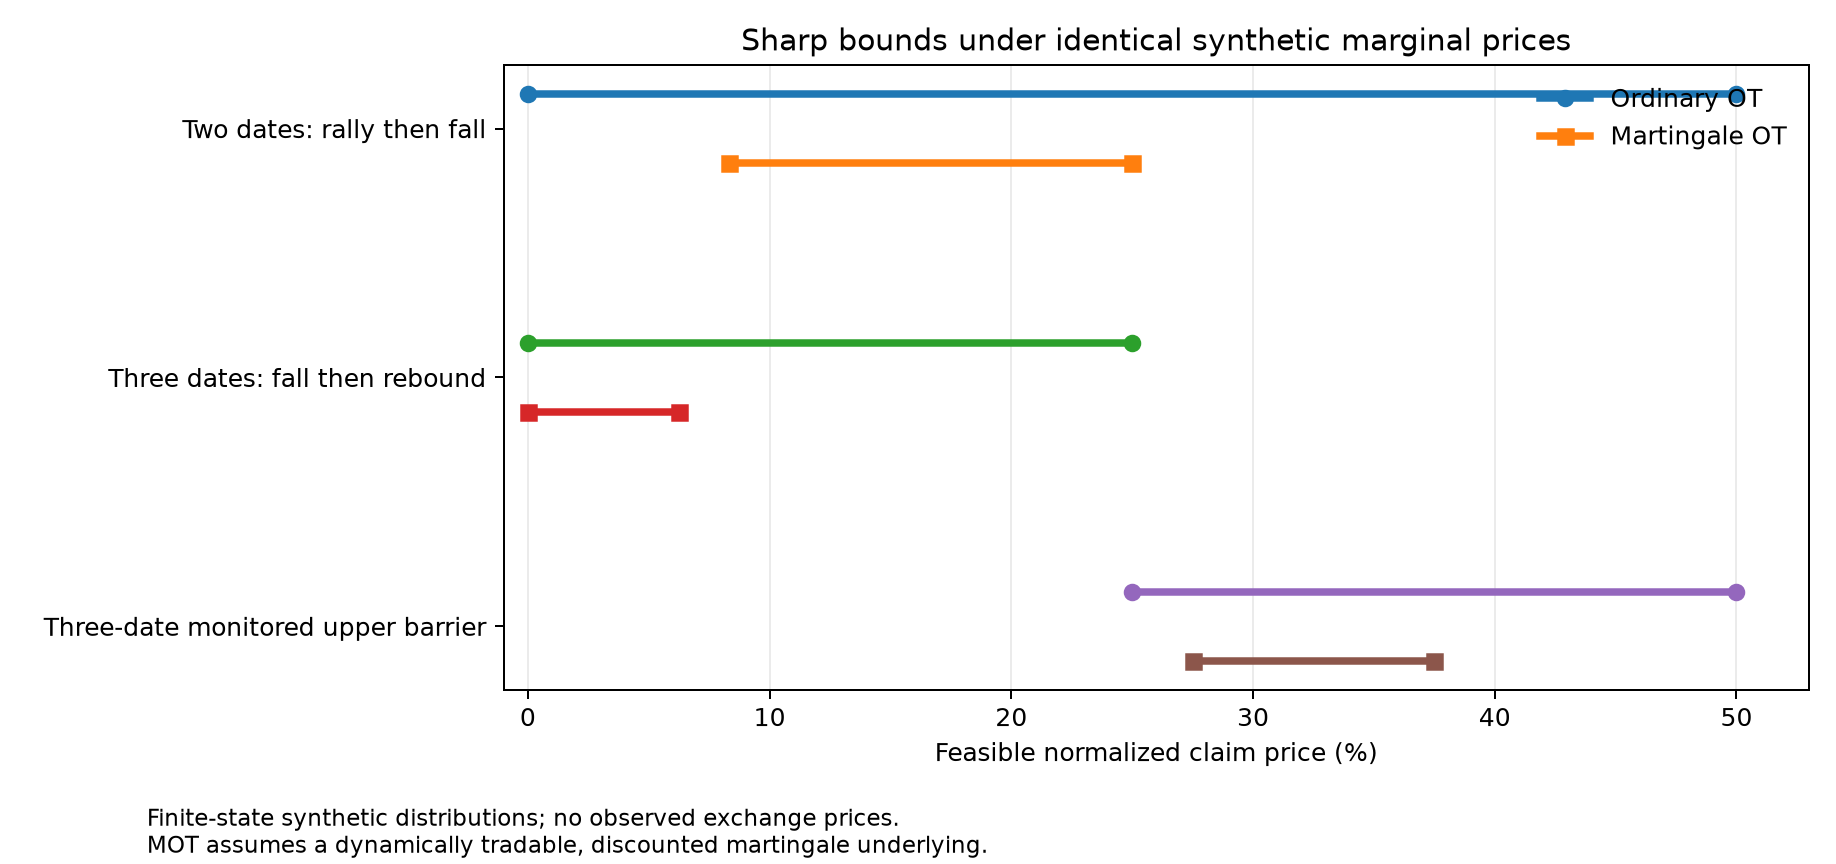
\includegraphics[width=\linewidth]{../outputs/figures/transport_bound_comparison.png}
\caption{Sharp feasible intervals from synthetic marginal distributions. The
martingale restriction changes the set of admissible path laws and requires
an appropriately discounted, dynamically traded underlying.}
\label{fig:intervals}
\end{figure}

\section{Research scope and non-novelty guardrails}
Martingale OT and robust path-dependent option pricing are established
\citep{beiglbock2013model,guo2021path,engstrom2025computation}.
Adapted transport and robust multicausal hedging have also been studied
\citep{krsek2025general}. Recent prediction-market work already treats
logical combinatorial arbitrage \citep{shi2026combinatorial} and coherent
joint parlay market making \citep{rana2026parlay}. Accordingly, neither
finite-state linear programming nor copula bounds constitutes a standalone
novelty claim. In the prediction-market setting, temporal arrival of
information should not be confused with an adapted-transport constraint:
the latter must specify \emph{which processes are coupled and what
information their coupling is allowed to use}.

\section{Falsifiable empirical agenda (not yet executed)}
\begin{enumerate}
\item Construct a settlement-semantics audit: oracle, event definition,
cutoff, observation schedule, currency, collateral, settlement lag.
\item Recover contract payoff vectors on compatible joint states; store
bid/ask/depth snapshots \emph{with timestamps}, not last-trade prices.
\item Compute successive intervals: singleton marginals, pairwise joints,
conditional claims, and (only for traded underlying) option-calibrated
martingale constraints.
\item Record interval width, interval contraction, model feasibility,
and executable bound violations after spread, size, fees and timing costs.
\item Hold out joint contracts for out-of-sample interval coverage and
compare entropy-regularized priors against maximum-entropy and parametric
copula baselines. Report lack of identification when the interval remains wide.
\end{enumerate}
No live order books or venue-level claims have been analyzed in this note.
All market inputs and numeric results are synthetic. The package is
research software, not a trading system or investment recommendation.

\section{Verification boundary}
The exact witness tables and dual coefficients are recorded in
\path{research/rational_certificates.md}. Reproducible checks are in
\path{tests/test_certificates.py}. A floating-point solver is used only
to propose candidate witnesses; rational reconstruction must pass every exact
constraint before being accepted. Lean 4.20.0 compiles the static three-event and two-date MOT sharp-bound
certificates over all real feasible laws; the audited dependencies are only
propositional extensionality, classical choice and quotient soundness.
The claim register records exact theorem names and build evidence. No general
Kantorovich or martingale strong-duality theorem, verified SciPy implementation,
continuous-time extension, or executable traded arbitrage is claimed.

% Self-contained bibliography for local builds without a BibTeX executable.
% references.bib is also supplied for later Overleaf/BibTeX migration.
\begin{thebibliography}{9}
\raggedright
\bibitem[Beiglbock et~al.(2013)]{beiglbock2013model}
M.~Beiglbock, P.~Henry-Labordere, and F.~Penkner.
Model-independent bounds for option prices---a mass transport approach.
\emph{Finance and Stochastics}, 17(3):477--501, 2013.
\href{https://doi.org/10.1007/s00780-013-0205-8}{doi:10.1007/s00780-013-0205-8}.
\bibitem[Guo and Loeper(2021)]{guo2021path}
I.~Guo and G.~Loeper.
Path dependent optimal transport and model calibration on exotic derivatives.
\emph{The Annals of Applied Probability}, 31(3):1232--1263, 2021.
\href{https://doi.org/10.1214/20-AAP1617}{doi:10.1214/20-AAP1617}.
\bibitem[Engstrom et~al.(2025)]{engstrom2025computation}
L.~Engstrom, S.~Kallblad, and J.~Karlsson.
Computation of robust option prices via structured multimarginal martingale
optimal transport. \emph{SIAM Journal on Financial Mathematics}, 2025.
\href{https://doi.org/10.1137/24M1670573}{doi:10.1137/24M1670573}.
\bibitem[Krsek and Pammer(2025)]{krsek2025general}
D.~Krsek and G.~Pammer.
General duality and dual attainment for adapted transport.
\emph{Applied Mathematics and Optimization}, 91(2), 2025.
\href{https://doi.org/10.1007/s00245-025-10240-y}{doi:10.1007/s00245-025-10240-y}.
\bibitem[Rana et~al.(2026)]{rana2026parlay}
R.~Rana, V.~Nadkarni, N.~Moshrefi, and P.~Viswanath.
ParlayMarket: Automated market making for parlay-style joint contracts.
2026. \url{https://arxiv.org/abs/2603.22596}.
\bibitem[Shi and Zhai(2026)]{shi2026combinatorial}
H.~Shi and D.~Zhai.
Combinatorial arbitrage in prediction markets.
2026. \url{https://arxiv.org/abs/2610.23517}.
\bibitem[Conditional Tokens contributors(2026)]{gnosisconditional}
Conditional Tokens Documentation: Developer Guide.
\url{https://conditional-tokens.readthedocs.io/en/latest/developer-guide.html}.
Accessed October 29, 2026.
\end{thebibliography}
\end{document}
